%!TeX root=../tese.tex
%("dica" para o editor de texto: este arquivo é parte de um documento maior)
% para saber mais: https://tex.stackexchange.com/q/78101

%% ------------------------------------------------------------------------- %%

% "\chapter" cria um capítulo com número e o coloca no sumário; "\chapter*"
% cria um capítulo sem número e não o coloca no sumário. A introdução não
% deve ser numerada, mas deve aparecer no sumário. Por conta disso, este
% modelo define o comando "\chapter**".
\chapter{Introdução}
\label{cap:introducao}

\enlargethispage{.5\baselineskip}

Grafos são estruturas de dados que nos permitem modelar vários problemas existentes da vida real, sejam eles estáticos ou dinâmicos. Em problemas estáticos, o grafo não sofre alterações com o passar do tempo. Podemos citar, como exemplo, o planejamento de rotas de entrega, análise de moléculas químicas e de dependências em software utilizando ordenação topológica. Entretanto, ainda existem muitas situações em que ocorre dinamicidade, como nas interações de usuários em redes sociais, monitoramento de epidemias (contatos e isolamentos) e sistemas de navegação \textit{GPS}, onde há necessidade de recalcular rotas dependendo das condições como congestionamentos e acidentes. Para modelar tais problemas, usamos grafos dinâmicos para modelá-los.

Dessa forma, são considerados problemas em grafos completamente dinâmicos aqueles em que o grafo sofre, com o tempo, alterações como inserções e remoções 
de arestas. Caso o algoritmo permita apenas inserção ou apenas remoção, tais 
problemas são chamados de parcialmente dinâmicos, conforme Holm, de Lichtenberg e Thorup ~\cite{jacob_holm}. Note que as operações de 
atualização e consulta são apresentadas de forma online, sem conhecimento algum das operações futuras.

Aqui serão tratados problemas em que o grafo dinâmico possui um conjunto fixo de vértices \textit{V}, e estabelecemos $n = |\textit{V}\ |$. Além disso, pode-se definir $m$ como o número de arestas existentes. Na maior parte das vezes, a complexidade de tempo das operações será amortizada, o que implica que elas são calculadas como a média sobre todas as operações realizadas. 

Um grafo dinâmico de ordem $n$ é uma sequência de grafos ($G_0$, $G_1$, $\ldots$, $G_T$), onde $G_0$ é o grafo inicial com \textit{n} vértices e cada $G_t$ para $1 \leq t \leq T$ é obtido a partir de $G_{t-1}$ pela adição ou remoção de alguma aresta. Chamamos de \textbf{alteração}, \textbf{modificação} ou \textbf{atualização} quando ocorre alguma operação de adição e/ou remoção de arestas no grafo dinâmico.

Um problema em grafos dinâmicos consiste em verificar se o grafo atual \textit{G} satisfaz alguma propriedade, e cada operação que realiza essa verificação é denominada \textbf{consulta}. A solução do problema depende da criação de um algoritmo que utiliza uma estrutura de dados capaz de realizar estas consultas e as alterações de forma eficiente. 

Iremos tratar inicialmente do \textbf{problema de conexidade em grafos dinâmicos}, que consiste em manter um grafo dinâmico que sofre uma sequência de inserções e remoções de arestas. Entre essas modificações, realizamos consultas para verificar se dois vértices \textit{u} e \textit{v} estão conectados por algum caminho. Porém, antes de entrarmos em detalhes, iremos apresentar alguns conceitos importantes que constituirão a base do nosso problema. 

Uma \textbf{floresta} em um grafo $G$ é um subgrafo acíclico de $G$. Uma \textbf{árvore} é uma floresta conexa, ou seja, uma floresta pode conter várias árvores desconexas. Um subgrafo $F$ de $G$ é gerador se contém todos os vértices de $G$. Com isso, podemos enunciar um problema clássico em grafos chamado o problema da árvore geradora de custo mínimo (MST, de \textit{Minimum Spanning Tree}). Seja um grafo conexo $G = (V, E)$, onde $V$ é o conjunto de vértices e $E$ o conjunto de arestas. Para cada aresta $uv \in E$, temos um peso $w(uv)$ associado. Assim, o objetivo do problema é encontrar uma árvore geradora cujo peso total 

$$
w(T) = \sum_{e \,\in\, E(T)} w(e)
$$
seja mínimo. A Figura 1.1 mostra um exemplo de grafo conexo com pesos nas arestas e uma árvore geradora mínima de peso 17.

\begin{figure}
    \centering
    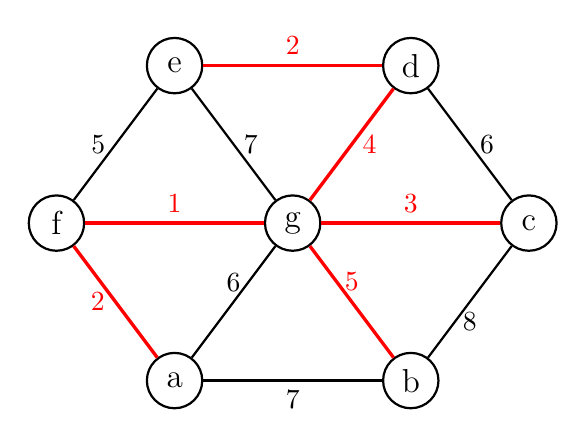
\begin{tikzpicture}
        [node/.style={circle,draw,minimum size=2em, thick, font=\large},
        edge/.style={thick},
        mst/.style={very thick, red}]
        
        % Vertices in a circular arrangement
        \node[node] (A) at (0,0) {a};
        \node[node] (B) at (3,0) {b};
        \node[node] (C) at (4.5,2) {c};
        \node[node] (D) at (3,4) {d};
        \node[node] (E) at (0,4) {e};
        \node[node] (F) at (-1.5,2) {f};
        \node[node] (G) at (1.5,2) {g};
        
        % Non-MST edges (normal black edges)
        \draw[edge] (A) -- (B) node[midway, below] {7};
        \draw[edge] (B) -- (C) node[midway, below] {8};
        \draw[edge] (C) -- (D) node[midway, right] {6};
        \draw[edge] (A) -- (G) node[midway, above] {6};
        \draw[edge] (E) -- (G) node[midway, right] {7};
        \draw[edge] (F) -- (E) node[midway, left] {5};
        
        % MST edges (highlighted in red)
        \draw[mst] (A) -- (F) node[midway, left] {2};
        \draw[mst] (G) -- (D) node[midway, right] {4};
        \draw[mst] (F) -- (G) node[midway, above] {1};
        \draw[mst] (G) -- (C) node[midway, above] {3};
        \draw[mst] (E) -- (D) node[midway, above] {2};
        \draw[mst] (B) -- (G) node[midway, above] {5};
        
    \end{tikzpicture}
    \caption{Um grafo com sete vértices. As arestas em vermelho formam uma árvore geradora mínima (MST) de peso total 17.}
    \label{fig:mst_example}
\end{figure}

Para encontrar uma árvore geradora mínima, podemos utilizar uma abordagem gulosa para o problema. Existem dois algoritmos gulosos clássicos que resolvem este problema eficientemente, quando o grafo não é dinâmico: o algoritmo de Kruskal e o de Prim. Cada um deles estabelece uma regra específica para determinar uma aresta segura.

Se um grafo $G$ tem $n$ vértices e $m$ arestas, o algoritmo de Kruskal consome O($m$lg$m$), que é a complexidade de tempo para ordenar as arestas em ordem crescente de peso. Já o algoritmo de Prim pode ser implementado de modo a consumir O($m$ + $n$lg$n$), usando Fibonacci heaps. Tais algoritmos e suas implementações estão bem descritos no Capítulo~23.2 do livro de Cormen, Leiserson, Rivest e Stein ~\cite{clrs}, não iremos aprofundá-los em nosso estudo. 

No nosso estudo, estamos interessados em grafos dinâmicos, que podem sofrer inserções e remoções de arestas, e por isso abrimos mão de exigir que o grafo seja conexo. Queremos manter uma floresta geradora maximal (MSF) de custo mínimo do grafo. Este problema já existe uma solução proposta por Holm, de Lichtenberg e Thorup~\cite{jacob_holm} na Seção~5 do seu artigo. Essa solução se baseia num algoritmo para o problema de conexidade em grafos dinâmicos, descrito na Seção~3 de seu artigo. 

No decorrer do nosso estudo, iremos destrinchar a solução dos autores em vários capítulos do texto. No Capítulo~2 descreveremos brevemente o problema da conexidade em grafos dinâmicos. No Capítulo~3: descreveremos a nossa implementação do algoritmo para o problema da floresta geradora maximal de custo mínimo decremental. No Capítulo~4...

As implementações dos nossos algoritmos da solução de \textit{Holm, de Lichtenberg e Thorup}~\cite{jacob_holm} serão feitas utilizando a linguagem \textit{C++}, onde disponibilizamos o código no repositório do \textit{GitHub} ~\cite{chung2025}.